\section{问题背景}

古代玻璃制品是早期中西方文化与贸易交流的重要物证。古代玻璃的主要成分为二氧化硅,为降低其熔点,制造过程中常需加入助熔剂。以草木灰为助熔剂得到高钾玻璃,而以铅矿石为助熔剂则得到铅钡玻璃,二者因制作工艺的差异导致化学成分构成不同,这也成为区分玻璃来源的依据。因此,通过分析玻璃文物样本的化学成分,能够为考古学研究提供有价值的参考信息。

玻璃制品在长期埋藏过程中会发生风化现象,其内部元素与环境发生交换,导致表面化学成分比例改变。风化作用的存在为依据化学成分鉴别玻璃类型带来了挑战。部分文物表面风化严重,其现有成分数据已不能直接反映其初始状态。如何利用已有数据,建立风化影响下玻璃分类的数学模型,并对风化过程进行定量分析,是本研究需要解决的核心科学问题。


% \begin{figure}[htbp]
%     \centering
%     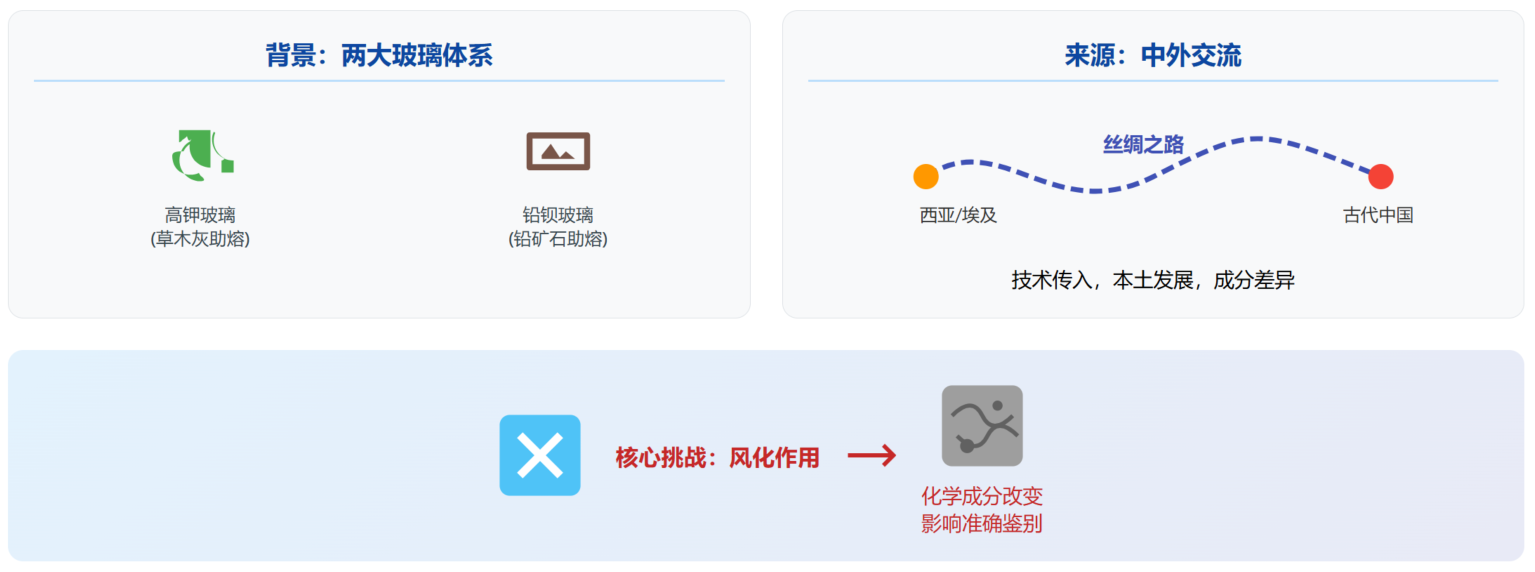
\includegraphics[width=\textwidth]{figs/1前置/问题背景.png}
%     \caption{问题背景} 
%     \label{fig:your_image_label} 
% \end{figure}


\section{问题重述}

\textbf{问题一}:分析表面风化与玻璃物理属性的关联,研究风化对不同类型玻璃化学成分的影响规律,并构建模型预测文物风化前的成分含量。

\textbf{问题二}:建立高钾玻璃与铅钡玻璃的分类模型,并对两大类玻璃进行亚类划分,同时分析划分结果的合理性与敏感性。

\textbf{问题三}:应用已建立的分类模型鉴别未知类别玻璃文物的所属类型,并进行敏感性分析。

\textbf{问题四}:分析不同类别玻璃内部各化学成分间的关联模式,并比较这些模式在不同类别间的差异。

\section{问题分析}

针对问题一,该问题涉及两个层面,其一是定性关系的判断,其二是定量规律的分析与预测。表面风化与玻璃类型、纹饰、颜色均为分类变量,它们之间的关联性分析适合采用非参数的卡方检验。风化对化学成分含量的影响则需要分组进行统计比较,通过观察含量分布的变化来识别规律。由于缺乏同一文物风化前后的成对数据,直接建立回归预测模型存在困难,因此分析的重点在于依据风化机理,构建一个基于平均变化率的风化系数模型,用以反推风化前的化学成分。

针对问题二,该问题需要从监督学习与无监督学习两个角度展开。高钾与铅钡玻璃的分类规律研究是一个典型的二分类问题,可以基于探索性数据分析发现的关键化学成分,构建支持向量机等分类模型,并对模型进行解释。亚类划分则是在已知大类的基础上进行更细致的探索,属于无监督聚类问题,需要先选择类内变异性高的化学成分作为特征,再运用层次聚类与轮廓系数等方法确定最优的亚类数量,最后对划分结果进行化学特征解释与敏感性分析。

针对问题三,该问题是分类模型的实际应用与可靠性验证。分析的核心在于构建一个泛化能力强且稳健的分类器。这需要比较多种模型架构,并论证选择支持向量机的合理性。为使模型性能最优化,需要采用改进遗传算法等智能优化算法进行超参数寻优。最终的鉴别结果需要通过数据扰动和模型参数敏感性分析的双重检验,以证明其结论并非偶然,而是具有高度的可靠性。

针对问题四,该问题要求探寻不同类别玻璃内部化学成分的关联结构。由于玻璃成分数据具有总和恒定的特性,直接计算相关系数会产生误导,因此必须首先采用中心化对数比变换来消除此统计约束。变换之后,应使用图套索等方法计算能反映直接关联的偏相关系数,并构建网络。通过对网络进行社群发现与核心节点分析,可以将复杂的关联关系简化为宏观结构,从而比较两类玻璃在配方原理上的差异。


\section{模型假设}
为保证模型构建的合理性与分析过程的严谨性,我们提出以下基本假设。
\begin{enumerate}
    \item 所有用于分析的数据均为成分总和在百分之八十五至一百零五区间的有效数据。
    \item 数据中的空白项表示该化学成分未被检测到其含量可视为零。
    \item 同一类型玻璃的风化过程与化学成分变化规律具有统计上的一致性。
    \item 文物的化学成分组合能够有效地区分高钾玻璃与铅钡玻璃两大类别。
    \item 同一文物多个采样点的平均化学成分可以代表该文物的整体特征用于亚类划分。
    \item 化学成分间的偏相关关系能够反映其在玻璃配方或制作工艺中的直接关联。
\end{enumerate}

\section{符号说明}
本文后续章节中所使用的主要数学符号及其说明如表所示。

\begin{table}[H]
    \centering
    \caption{符号说明表}
    \begin{tabular}{ll}
        \toprule
        \textbf{符号} & \textbf{说明} \\
        \midrule
        $k_{t,j}$ & $t$类玻璃中$j$成分的风化系数 \\
        $\bar{C}_{t,j,\text{weathered}}$ & $t$类玻璃风化样本中$j$成分的平均含量 \\
        $\bar{C}_{t,j,\text{unweathered}}$ & $t$类玻璃未风化样本中$j$成分的平均含量 \\
        $C'_{\text{unweathered}, j}$ & 某一样本风化前$j$成分的预测含量 \\
        $\boldsymbol{w}, b$ & 支持向量机分类超平面的法向量与位移项 \\
        $C$ & 支持向量机的正则化系数 \\
        $\gamma$ & 径向基核函数的参数 \\
        $\xi_i$ & 支持向量机的松弛变量 \\
        $CV$ & 变异系数,用于衡量数据的相对离散程度 \\
        $\text{clr}(\boldsymbol{x})$ & 对样本向量$\boldsymbol{x}$进行中心化对数比变换 \\
        $S$ & 样本协方差矩阵 \\
        $\Theta$ & 精度矩阵,即逆协方差矩阵 \\
        $\lambda$ & 图套索算法的正则化参数 \\
        $\rho_{ij \cdot \text{rest}}$ & 变量$i$和$j$之间的偏相关系数 \\
        \bottomrule
    \end{tabular}
\end{table}